\clearpage
\section{Use cases}

\subsection{Use Case 1}

A user called testuser1 first sign up DAP market.

\begin{figure}[ht]
    \centering
    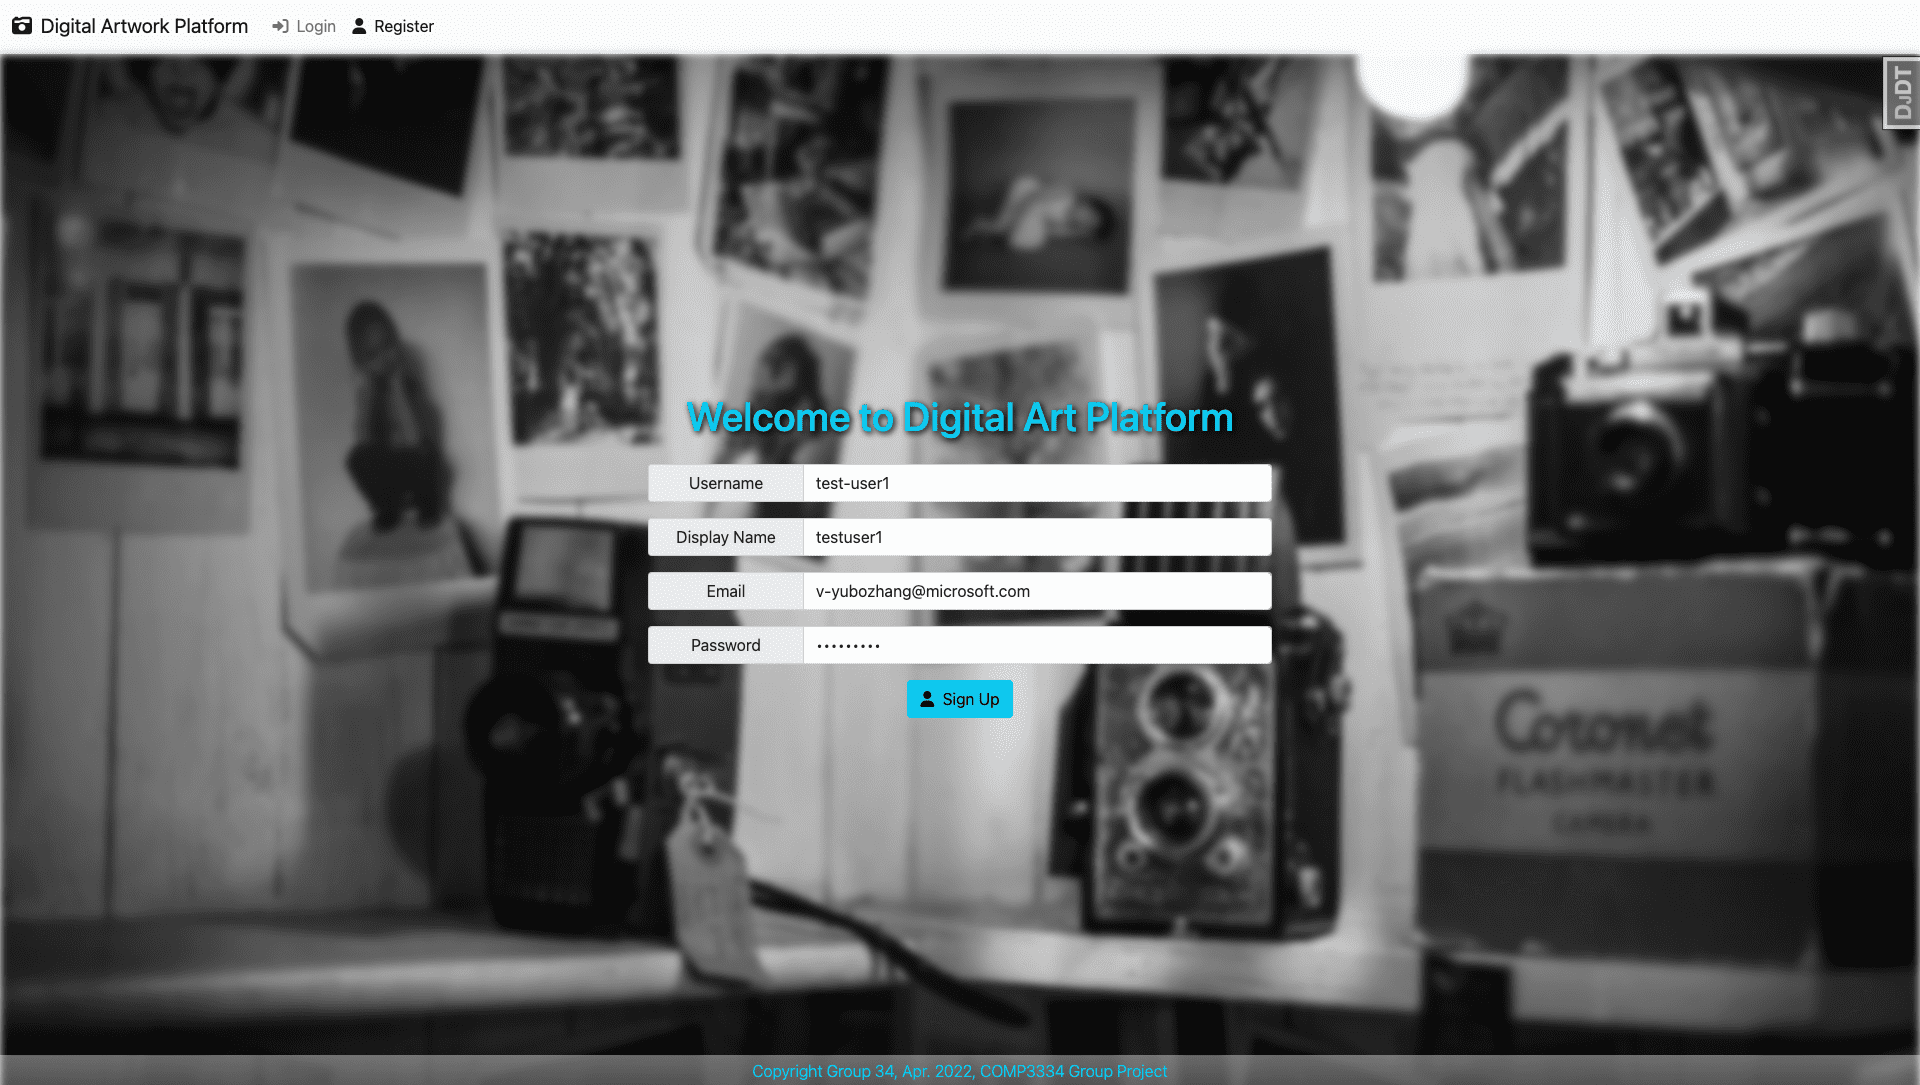
\includegraphics[width=0.7\linewidth]{figures/case1-2.png}
    \caption{Case1 -- Sign up}
    \label{fig: case1-2}
\end{figure}

After sign in, testuser1 can post his/her new digital artwork.

\begin{figure}[!h]
    \centering
    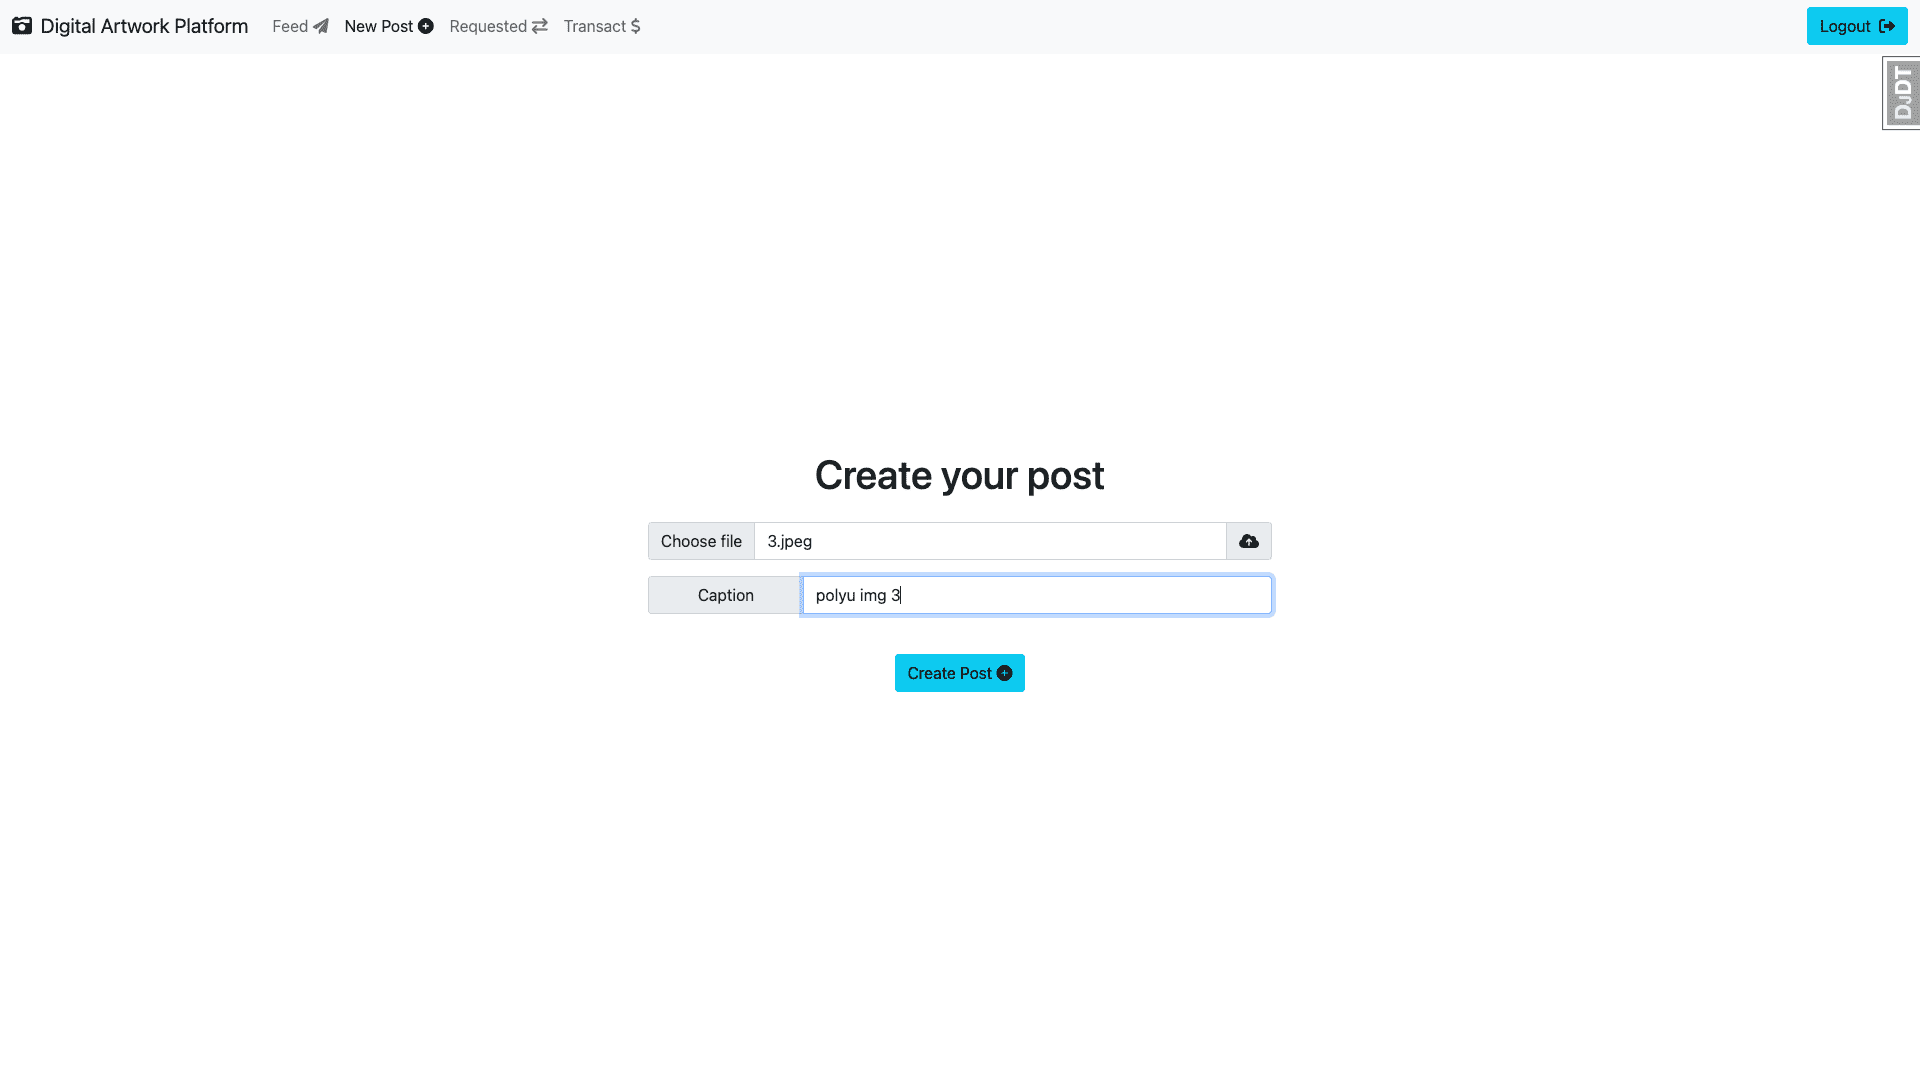
\includegraphics[width=0.8\linewidth]{figures/case1-3.png}
    \caption{Case1 -- Create your post.}
    \label{fig: case1-3}
\end{figure}

\begin{figure}[!h]
    \centering
    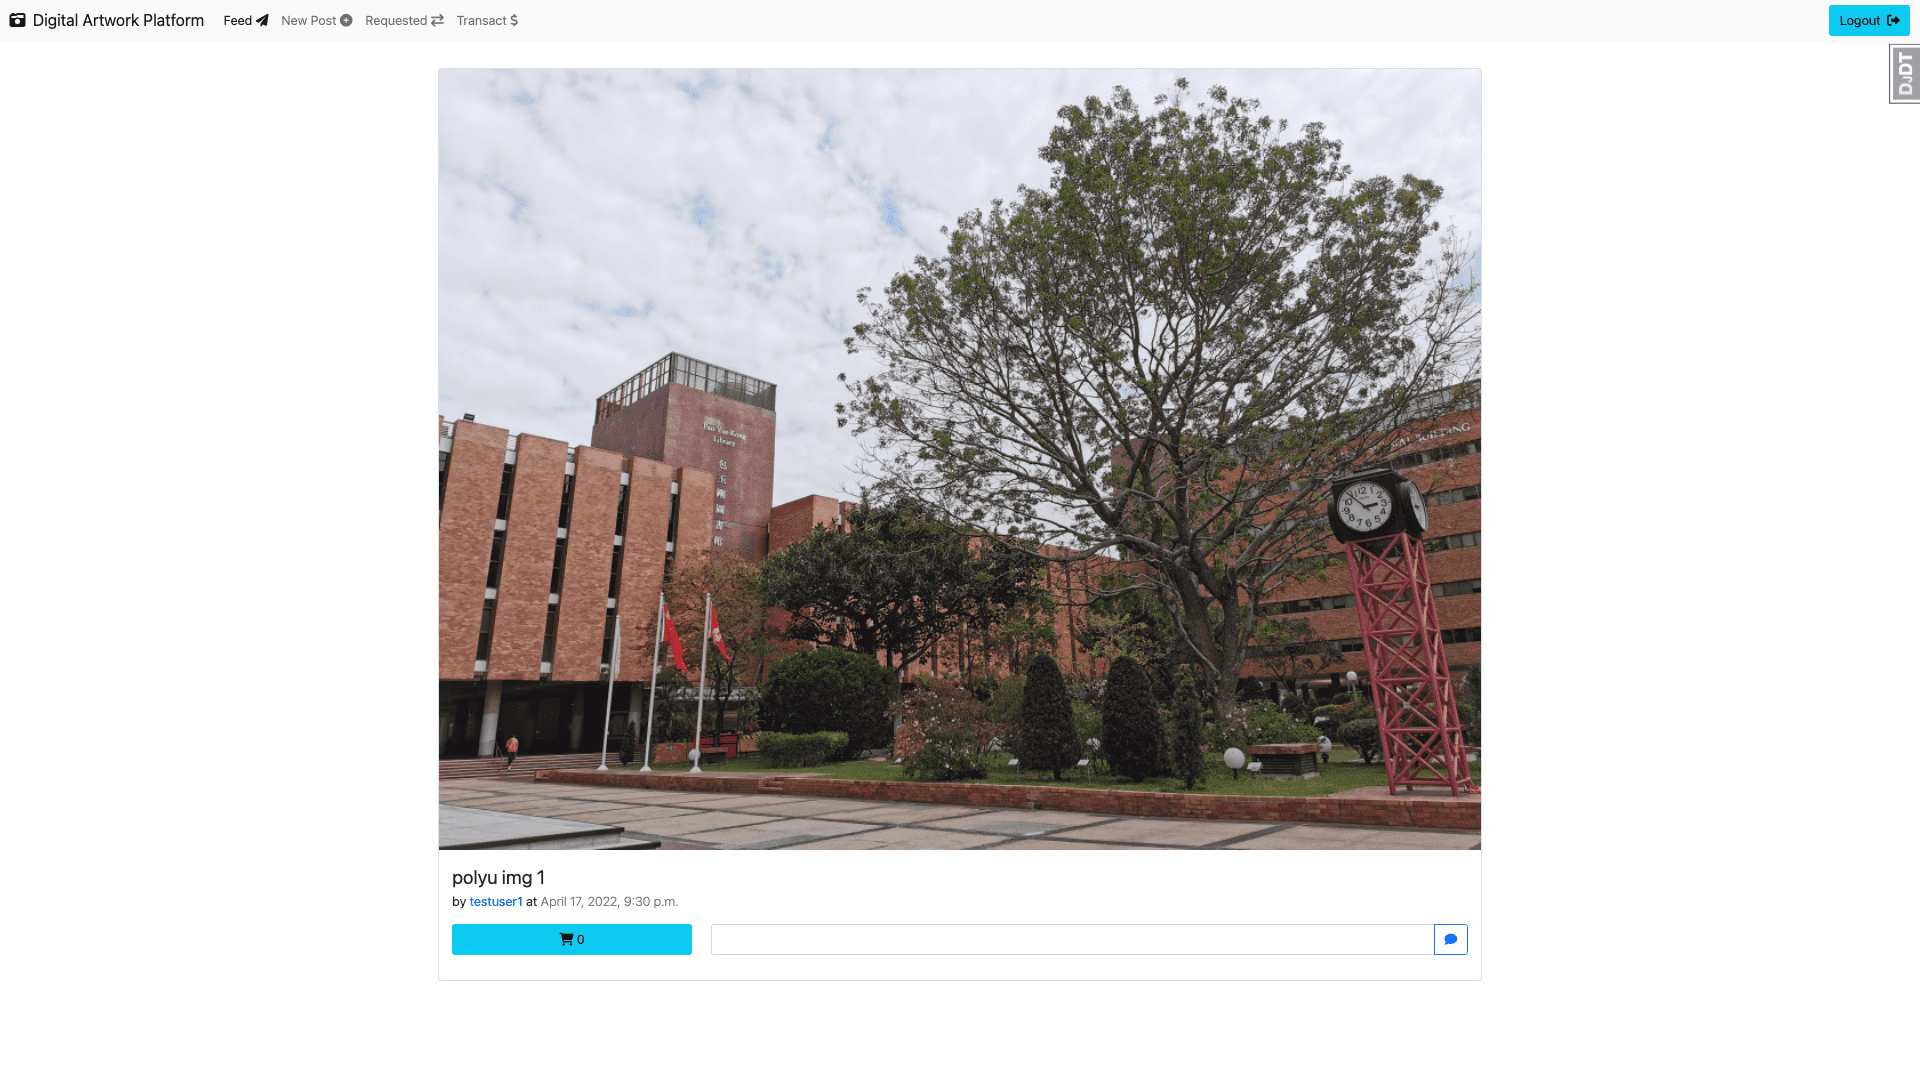
\includegraphics[width=0.8\linewidth]{figures/case1-4.png}
    \caption{Case1 -- View your created post.}
    \label{fig: case1-4}
\end{figure}

Similarly, another user called testuser2 can also sign up and then sign in to new a post. They can view other digital artworks at the "feed" page. 

\begin{figure}[!h]
    \centering
    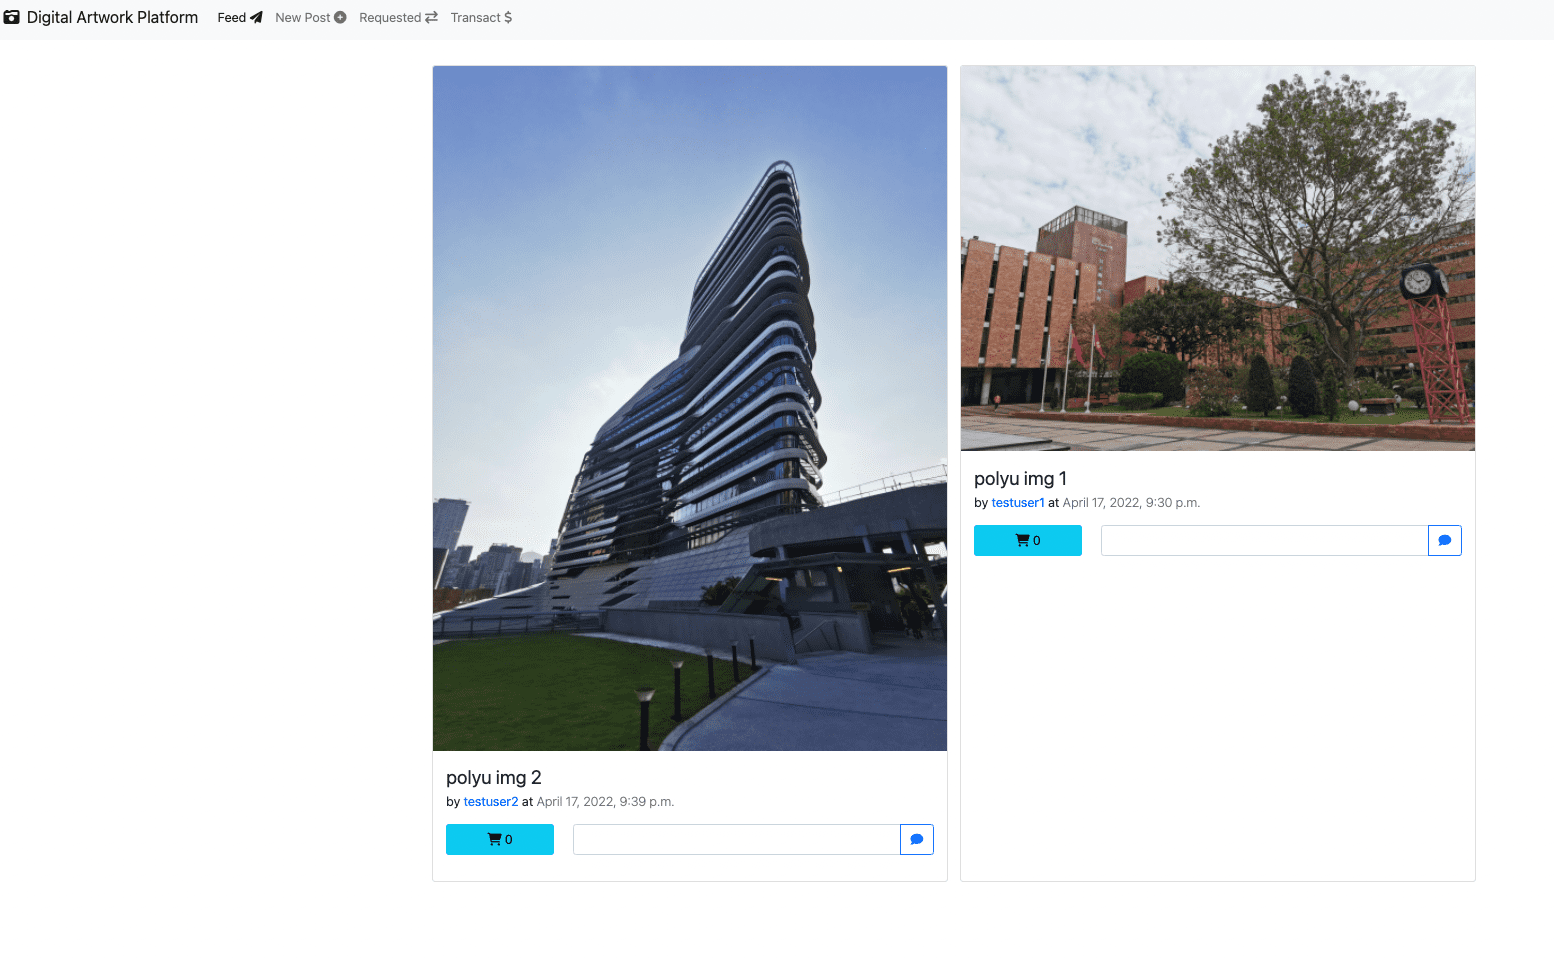
\includegraphics[width=0.9\linewidth]{figures/case1-5.png}
    \caption{Case1 -- Feed page with two digital artworks "polyu img 1" and "polyu img 2" created by testuser1 and testuser2 respectively.}
    \label{fig: case1-5}
\end{figure}

If testuser2 is intersted in testuser1's digital artwork "polyu img 1", he/she can press the "shopping cart" button and then a request will send to testuser1 via a encrypted system email.

\begin{figure}[h]
    \centering
    \begin{minipage}{.5\textwidth}
        \centering
        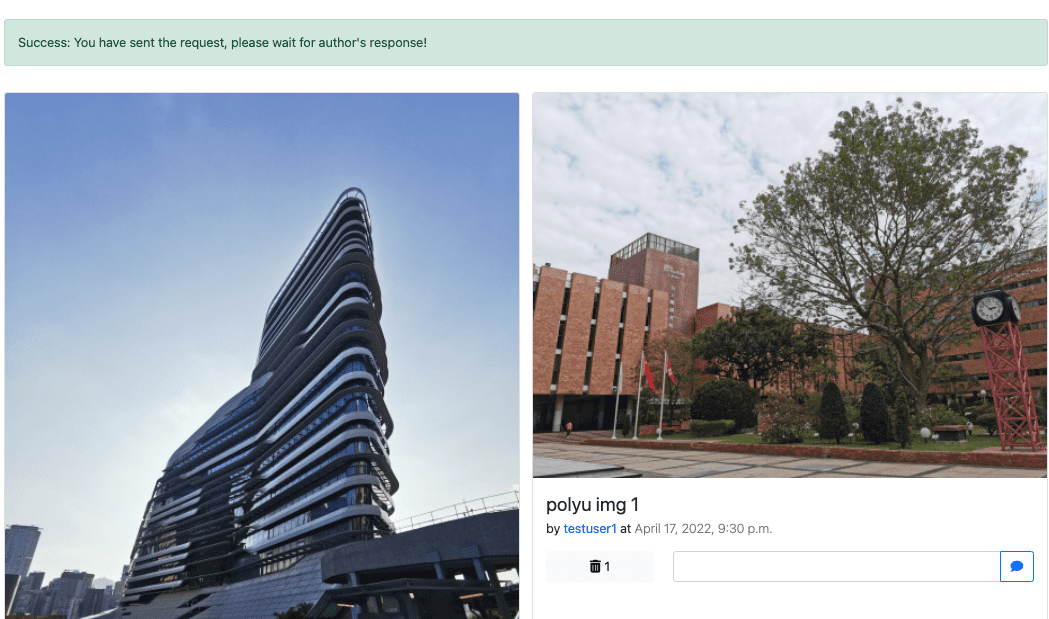
\includegraphics[width=\linewidth]{figures/case1-6.png}
        \caption{Case1 -- testuser2 send a request to testuser1's digital artwork "polyu img 1"}
        \label{fig: case1-5}
    \end{minipage}%
    \begin{minipage}{0.5\textwidth}
        \centering
        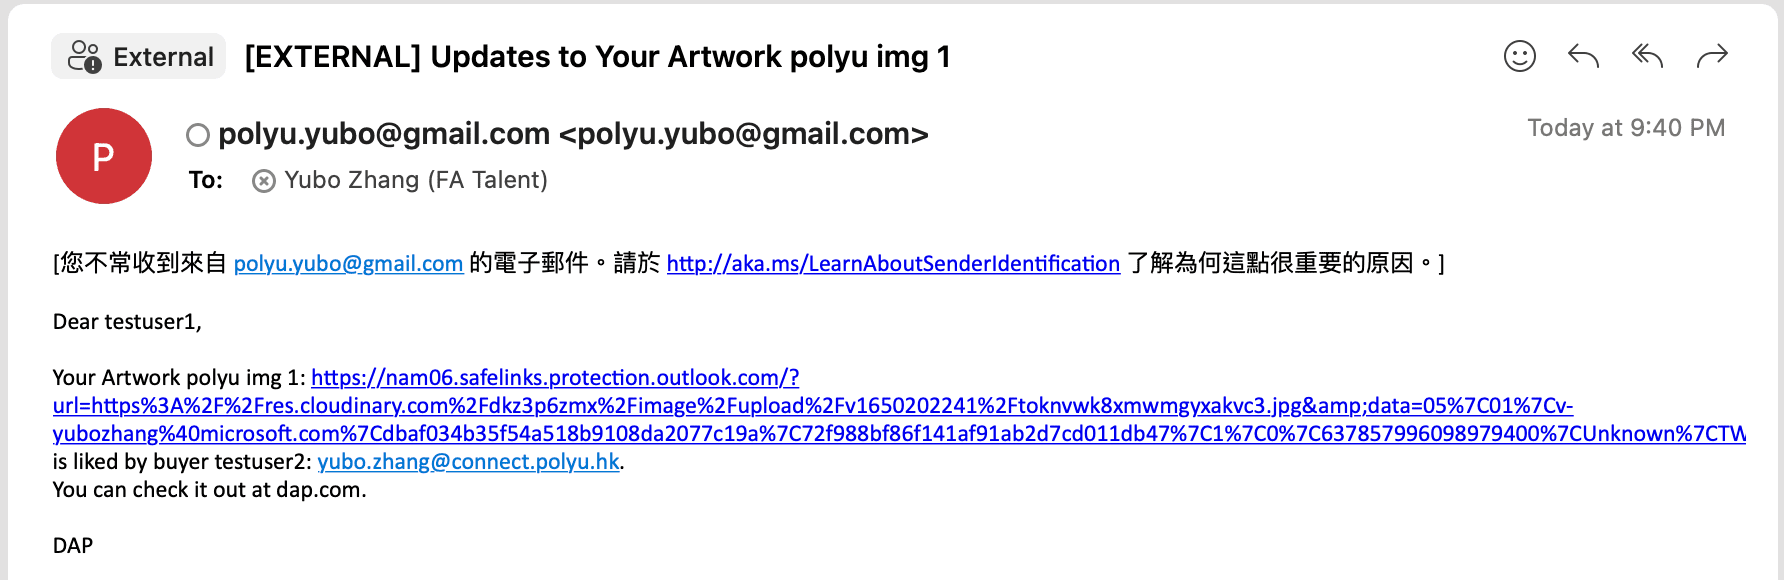
\includegraphics[width=\linewidth]{figures/case1-7.png}
        \caption{Case1 -- the email sent to testuser1}
        \label{fig: case1-6}
    \end{minipage}
\end{figure}

After testuser1 approved the transaction, testuser2 can checkout.

\begin{figure}[h]
    \centering
    \begin{minipage}{.5\textwidth}
        \centering
        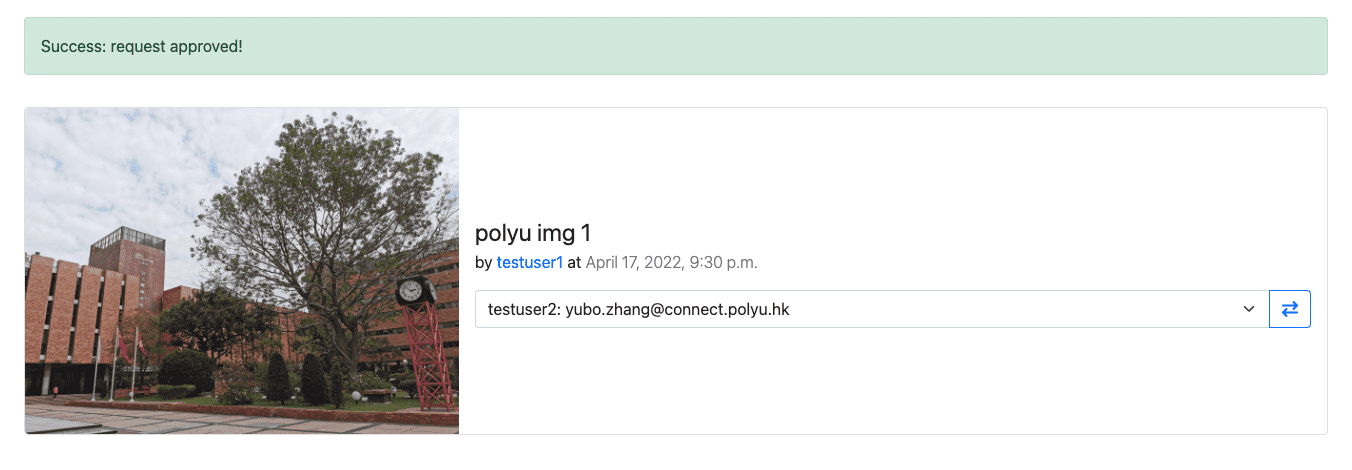
\includegraphics[width=\linewidth, heght=0.6\linewidth]{figures/case1-8.png}
        \caption{Case1 -- testuser1 approves the transaction}
        \label{fig: case1-5}
    \end{minipage}%
    \begin{minipage}{0.5\textwidth}
        \centering
        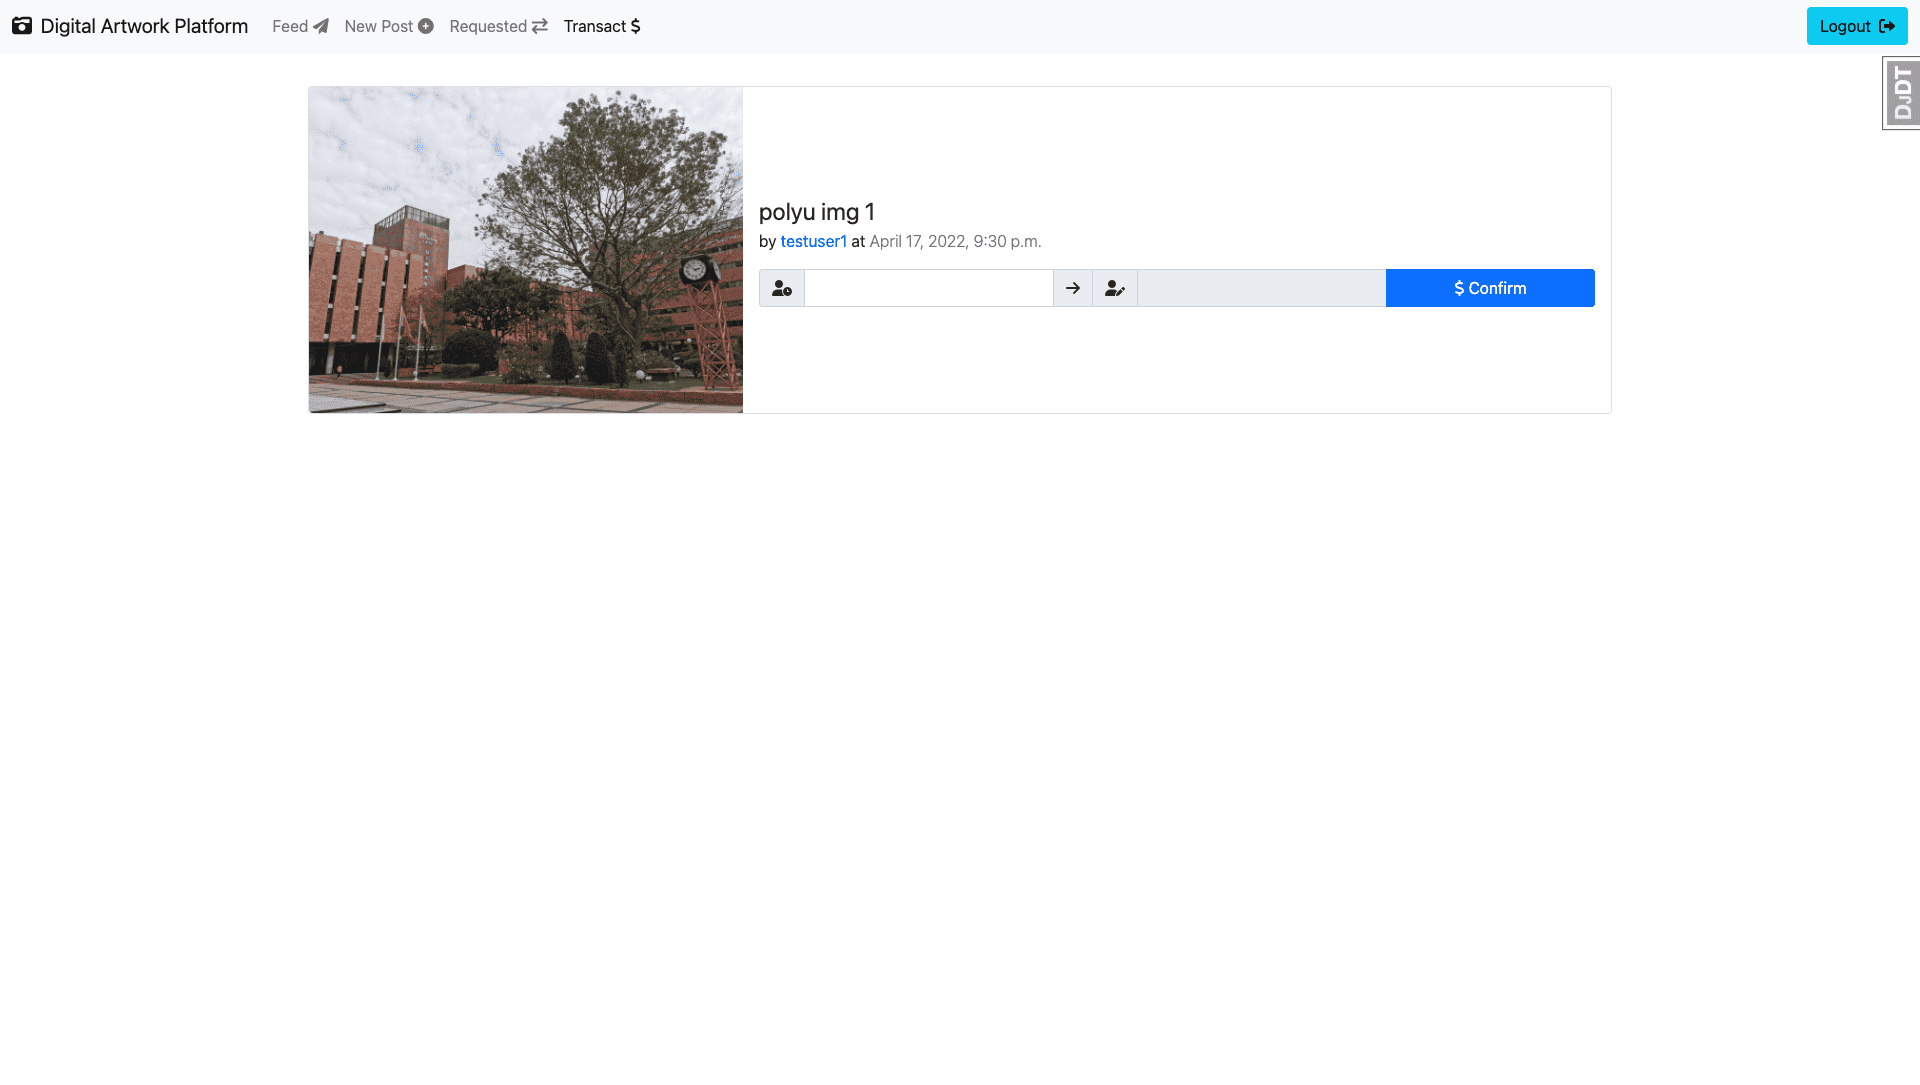
\includegraphics[width=\linewidth]{figures/case1-9.png}
        \caption{Case1 -- testuser1 checkout the transaction}
        \label{fig: case1-6}
    \end{minipage}
\end{figure}

Finally, the ownership of digital artwork "polyu img 1" is successfully changed to testuser2.
\clearpage

\begin{figure}[!h]
    \centering
    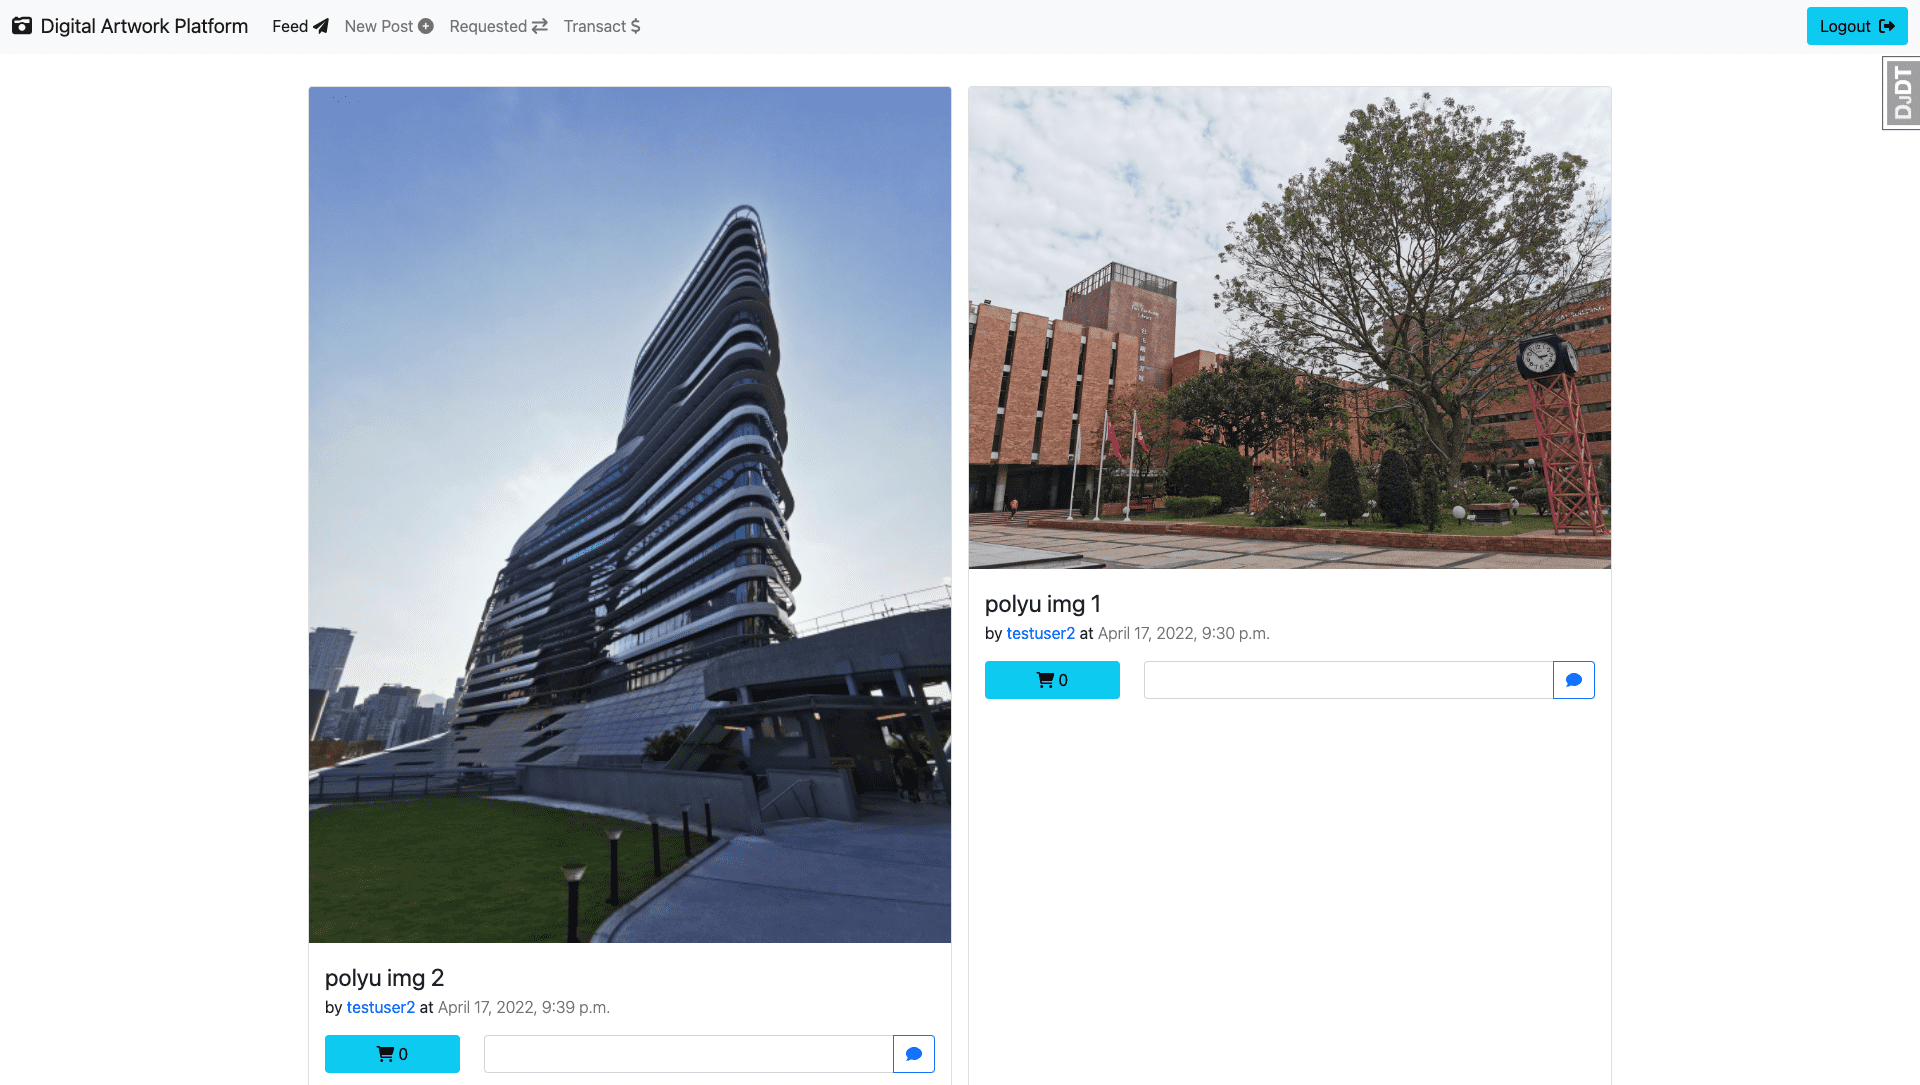
\includegraphics[width=0.75\linewidth]{figures/case1-10.png}
    \caption{Case1 -- Feed page with two digital artworks "polyu img 1" and "polyu img 2" created by testuser1 and testuser2 respectively.}
    \label{fig: case1-5}
\end{figure}

\vspace{-1cm}

\subsection{Use Case 2}

In this section, we will present some extra functions of DAP.

testuser1 posts a digital artwork called "polyu img 2". If testuser2 tries to upload a similar "copied" figure without testuser1's signature, DAP will warn him/her that this digital artwork already exists.

\begin{figure}[!h]
    \centering
    \begin{minipage}{.45\textwidth}
        \centering
        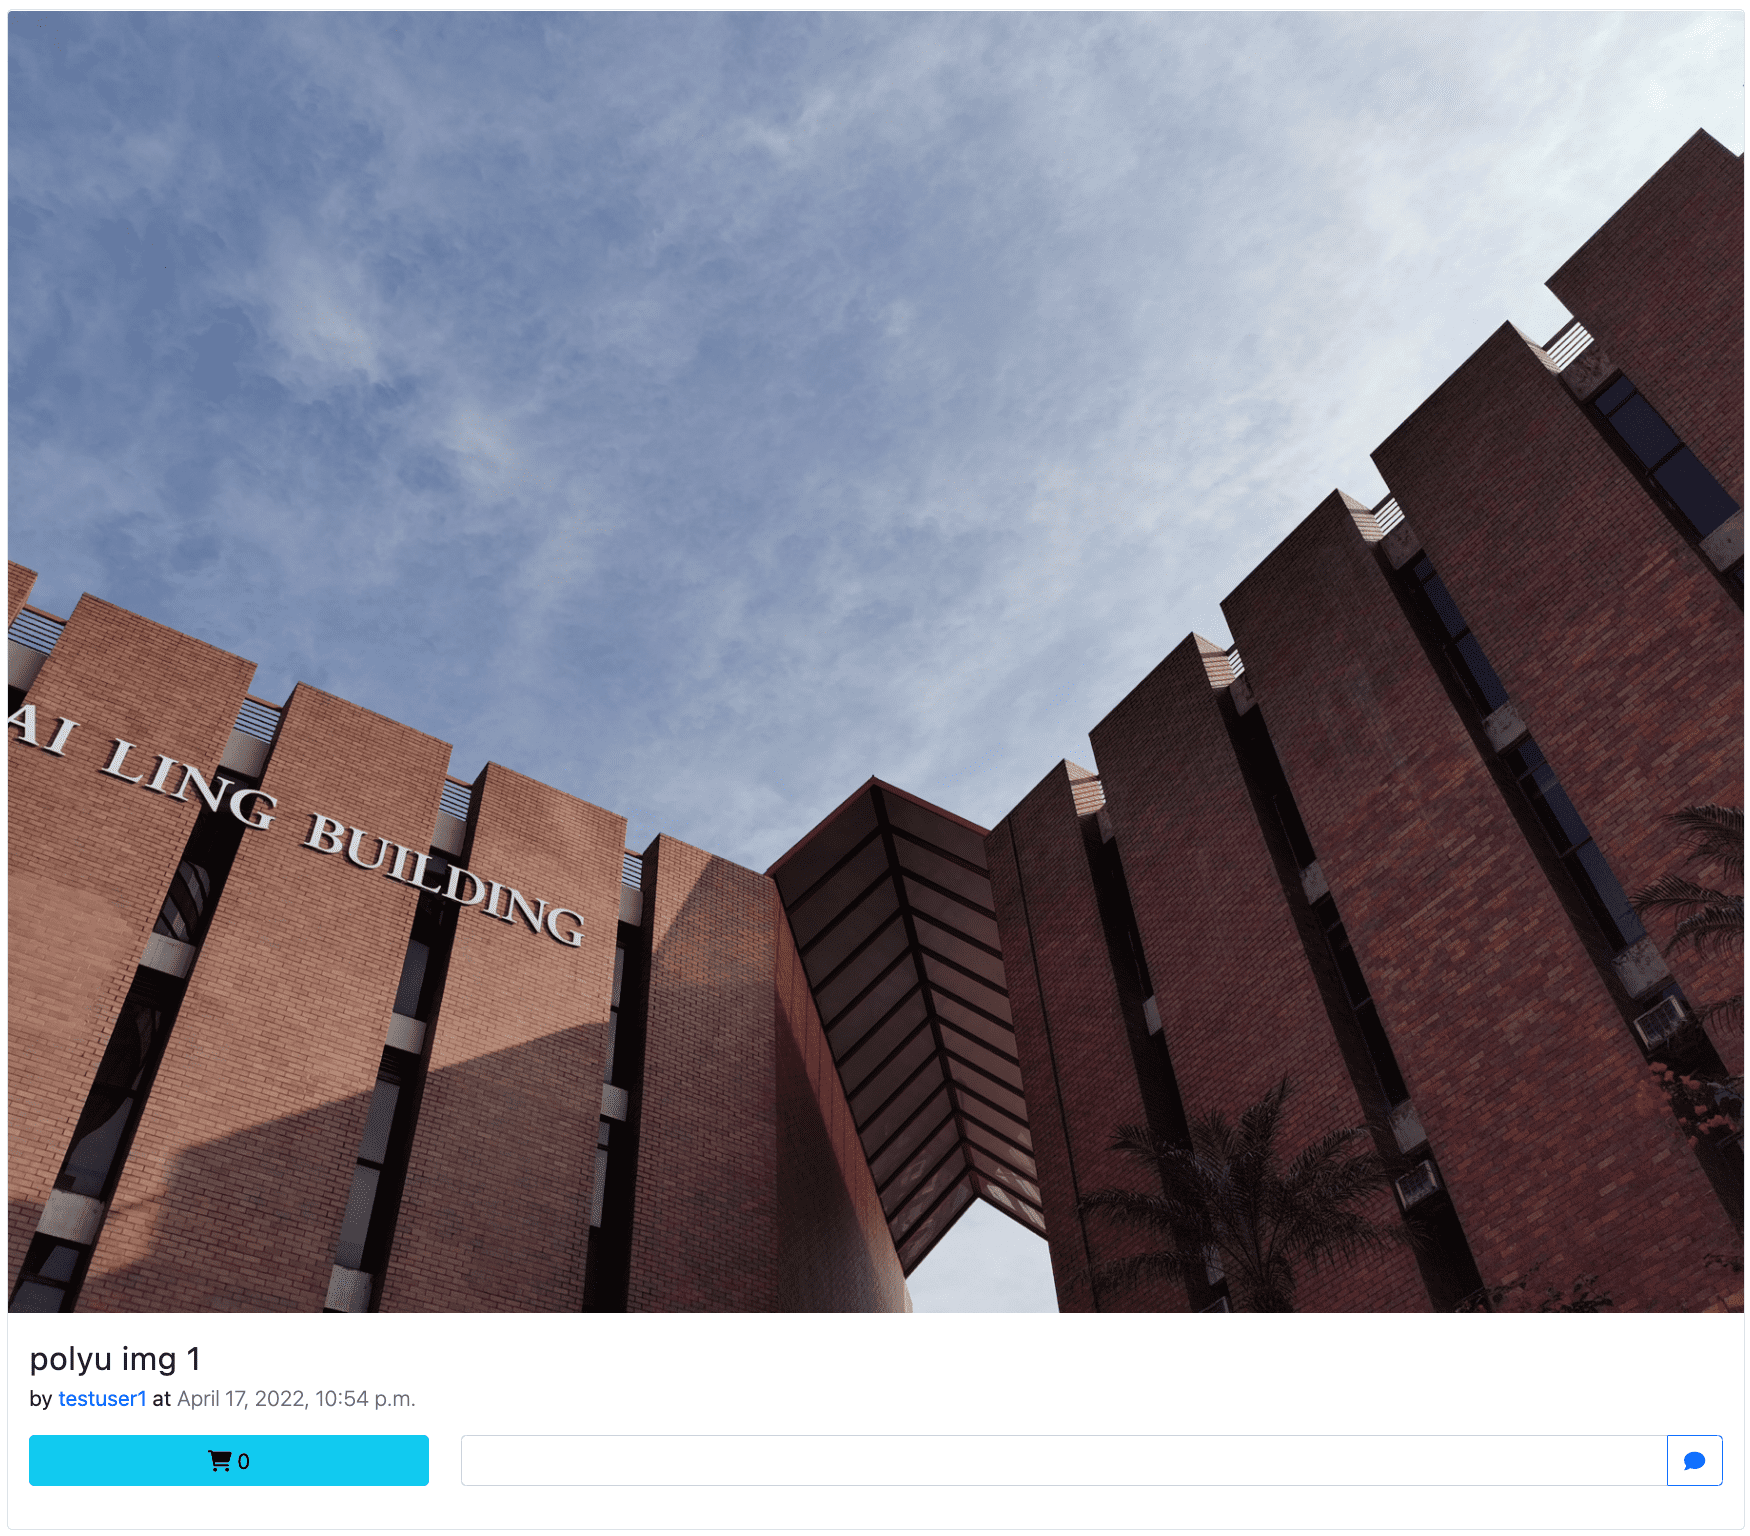
\includegraphics[width=\linewidth]{figures/case2-1.png}
        \caption{Case2 -- testuser1 post a digital artwork}
        \label{fig: case2-1}
    \end{minipage}%
    \begin{minipage}{0.45\textwidth}
        \centering
        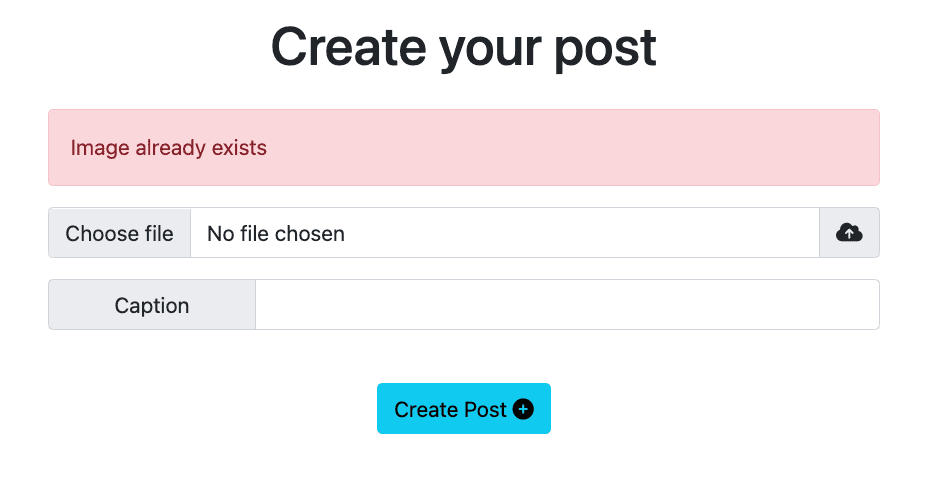
\includegraphics[width=\linewidth]{figures/case2-2.png}
        \caption{Case2 -- a warnning to testuser2}
        \label{fig: case2-1}
    \end{minipage}
\end{figure}

Besides sending "request" to the owner, testuser1 and testuser2 can also comment to show their interest. These comments are private and only visible to them.

\begin{figure}[!h]
    \centering
    \begin{minipage}{.5\textwidth}
        \centering
        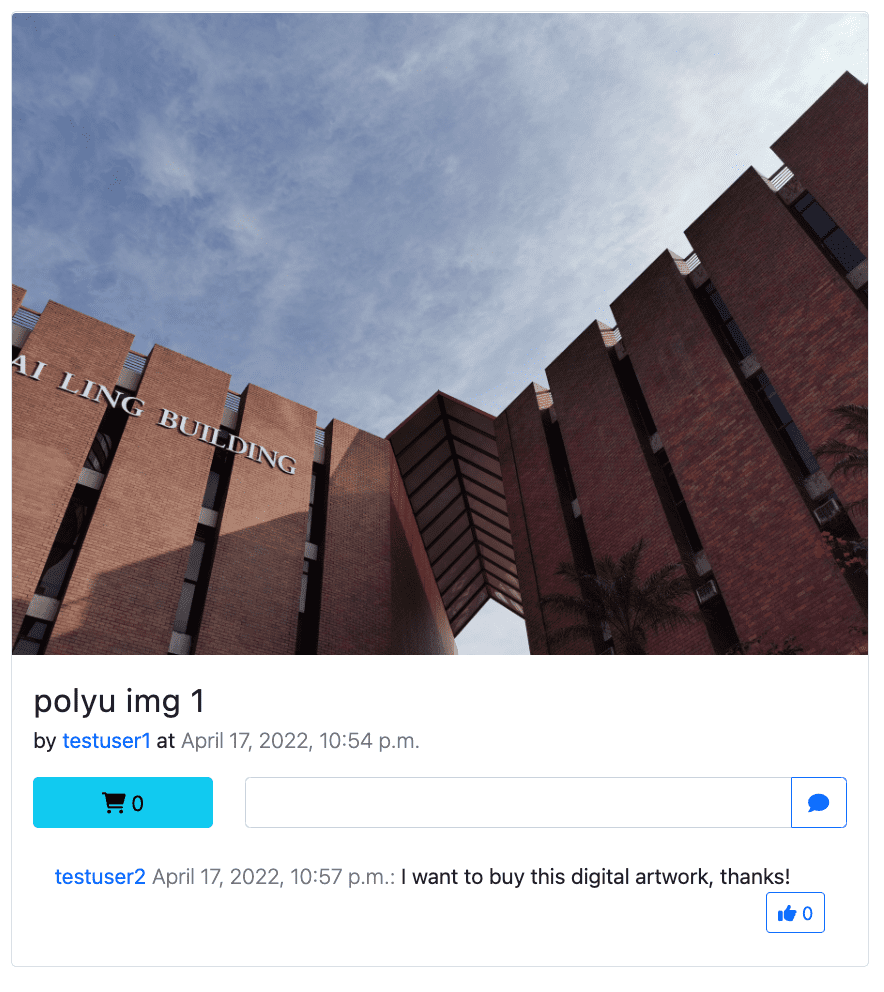
\includegraphics[width=\linewidth, height=\linewidth]{figures/case2-3.png}
        \caption{Case2 -- \\ testuser2 comment on "polyu img 1"}
        \label{fig: case2-1}
    \end{minipage}%
    \begin{minipage}{0.5\textwidth}
        \centering
        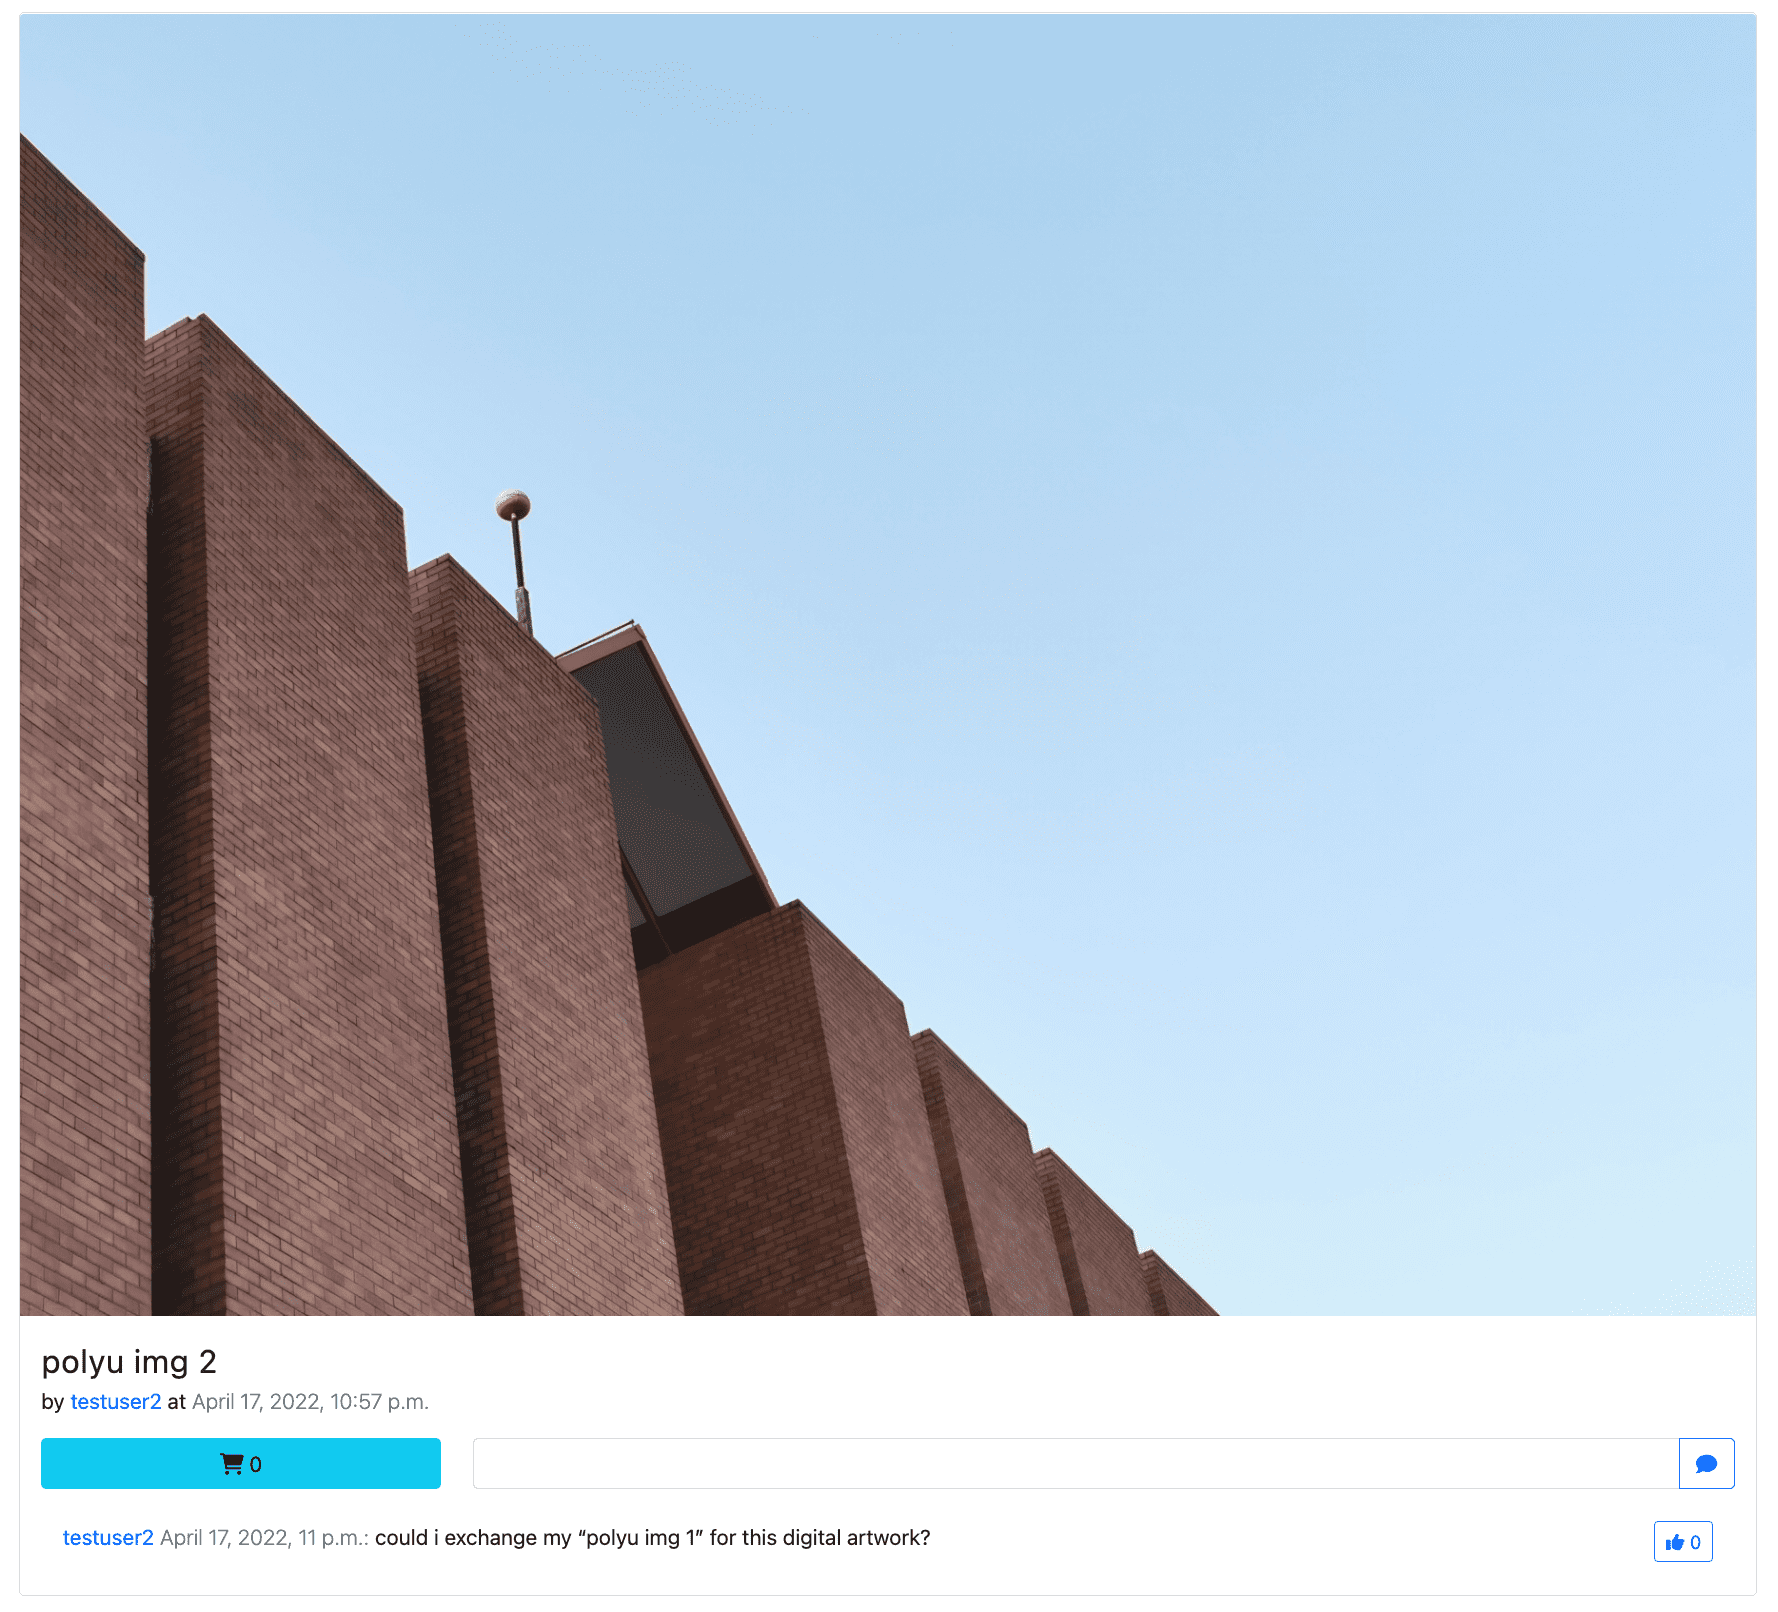
\includegraphics[width=\linewidth, height=\linewidth]{figures/case2-4.png}
        \caption{Case2 -- testuser1 reply via comment to testuser2}
        \label{fig: case2-1}
    \end{minipage}
\end{figure}

If they achieve agreement, they can complete the transaction procedure the same as case 1. After they both complete the transaction procedure, system check the transaction validity, then rewrite the ownership of their exchanged digital artworks.
